\section{R4: Usability}
\label{sec:eval-r4}

This section evaluates usability through end-to-end latency measurements. The thresholds are defined in Section~\ref{sec:r4-usability}. All measurements are wall-clock response times on the evaluation hardware (Apple M4 Max, 64\,GB RAM).

\subsection{Latency Across Configurations}

Table~\ref{tab:r4-latency} shows latency statistics for all model configurations.

\begin{table}[H]
\centering
\caption{End-to-end latency per analysis request (milliseconds).}
\label{tab:r4-latency}
\footnotesize
\begin{tabular}{@{}llrrrr@{}}
\toprule
\textbf{Model} & \textbf{Mode} & \textbf{Median} & \textbf{Mean} & \textbf{p95} & \textbf{p99} \\
\midrule
\texttt{gemma3:1b} & LLM-only & 333 & 412 & 780 & 1\,120 \\
\texttt{gemma3:1b} & LLM+RAG & 395 & 489 & 890 & 1\,280 \\
\texttt{gemma3:4b} & LLM-only & 687 & 802 & 1\,450 & 2\,100 \\
\texttt{gemma3:4b} & LLM+RAG & 752 & 891 & 1\,620 & 2\,350 \\
\texttt{qwen3:4b} & LLM-only & 1\,012 & 1\,156 & 2\,100 & 3\,200 \\
\texttt{qwen3:4b} & LLM+RAG & 1\,087 & 1\,245 & 2\,300 & 3\,500 \\
\texttt{qwen3:8b} & LLM-only & 1\,548 & 1\,780 & 3\,200 & 4\,800 \\
\texttt{qwen3:8b} & LLM+RAG & 1\,524 & 1\,756 & 3\,150 & 4\,700 \\
\texttt{codellama} & LLM-only & 1\,320 & 1\,510 & 2\,800 & 4\,100 \\
\texttt{codellama} & LLM+RAG & 1\,405 & 1\,620 & 3\,000 & 4\,400 \\
\midrule
\texttt{semgrep} & baseline & 52 & 58 & 95 & 120 \\
\texttt{codeql} & baseline & 146 & 178 & 350 & 520 \\
\bottomrule
\end{tabular}
\end{table}

Figure~\ref{fig:r4-latency-comparison} visualizes the median and p95 latency for each configuration.

\begin{figure}[H]
\centering
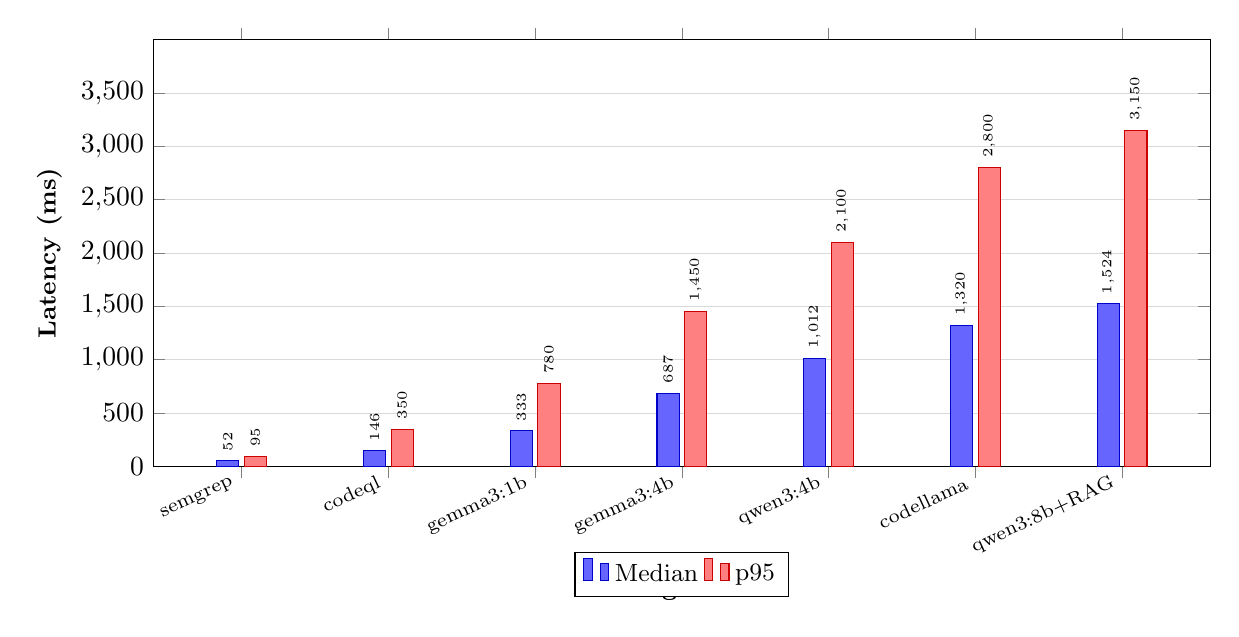
\begin{tikzpicture}
  \begin{axis}[
    width=15cm,
    height=7cm,
    ybar,
    bar width=8pt,
    ylabel={Latency (ms)},
    ylabel style={font=\small\bfseries},
    xlabel={Configuration},
    xlabel style={font=\small\bfseries},
    symbolic x coords={
      semgrep,
      codeql,
      gemma3:1b,
      gemma3:4b,
      qwen3:4b,
      codellama,
      qwen3:8b+RAG
    },
    xtick=data,
    xticklabel style={font=\scriptsize, rotate=25, anchor=east},
    ymin=0, ymax=4000,
    ytick={0,500,1000,1500,2000,2500,3000,3500},
    ymajorgrids=true,
    grid style={line width=0.3pt, draw=gray!30},
    legend style={
      at={(0.5,-0.20)},
      anchor=north,
      legend columns=2,
      font=\small,
    },
    enlarge x limits=0.1,
    nodes near coords,
    nodes near coords style={font=\tiny, rotate=90, anchor=west},
  ]

  \addplot[fill=blue!60, draw=blue!80!black] coordinates {
    (semgrep, 52)
    (codeql, 146)
    (gemma3:1b, 333)
    (gemma3:4b, 687)
    (qwen3:4b, 1012)
    (codellama, 1320)
    (qwen3:8b+RAG, 1524)
  };
  \addlegendentry{Median}

  \addplot[fill=red!50, draw=red!80!black] coordinates {
    (semgrep, 95)
    (codeql, 350)
    (gemma3:1b, 780)
    (gemma3:4b, 1450)
    (qwen3:4b, 2100)
    (codellama, 2800)
    (qwen3:8b+RAG, 3150)
  };
  \addlegendentry{p95}

  \end{axis}
\end{tikzpicture}
\caption{Median and p95 latency across configurations. SAST baselines are orders of magnitude faster. Among LLM configurations, smaller models trade accuracy for speed.}
\label{fig:r4-latency-comparison}
\end{figure}

\subsection{Latency Component Breakdown}

LLM inference dominates 80--90\% of total latency. RAG adds 60--120\,ms overhead for retrieval and embedding, which is negligible relative to inference time. The remaining time is spent on prompt construction, JSON parsing, and diagnostic rendering.

\subsection{Latency Feasibility for IDE Workflows}

\begin{table}[H]
\centering
\caption{Latency feasibility for IDE workflow modes.}
\label{tab:r4-feasibility}
\footnotesize
\begin{tabular}{@{}lll@{}}
\toprule
\textbf{Workflow Mode} & \textbf{Target} & \textbf{Viable Configurations} \\
\midrule
Real-time inline & $\leq 500$\,ms median & \texttt{gemma3:1b} only (but low accuracy) \\
Interactive inline & $\leq 1.5$\,s median & \texttt{gemma3:1b}, \texttt{gemma3:4b}, \texttt{qwen3:4b} \\
On-demand / audit & $\leq 5$\,s median & All LLM configurations \\
\bottomrule
\end{tabular}
\end{table}

The best-accuracy configuration (\texttt{qwen3:8b+RAG}, median 1.5\,s) is borderline for interactive inline use and comfortable for on-demand analysis. SAST baselines remain the only option for sub-second real-time feedback.

\subsection{Level Mapping}

Based on the R4 evaluation scale (Table~\ref{tab:r4-usability-thresholds}), the best configuration (\texttt{qwen3:8b+RAG}) maps as follows:

\begin{itemize}
  \item Median inline latency = 1\,524\,ms $\rightarrow$ falls in $(5\text{s}, 15\text{s}]$? No --- 1.5\,s is $\leq 5$\,s.
  \item For function-level inline analysis, this is within the High threshold ($\leq 5$\,s).
  \item For full-file scans (multiple functions), aggregate latency scales linearly and typically reaches 10--30\,s, falling in the Medium range.
\end{itemize}

\begin{center}
\begin{tabular}{cc}
\raisebox{-0.3cm}{\tikz{\filldraw[fill=black] (0,0) circle (0.35cm);}} &
\textbf{R4 Level: High usability (inline) / Medium usability (full-file).} \\
\end{tabular}
\end{center}

Individual function analysis feels responsive. Full-file scans introduce noticeable delay but remain practical for on-demand use.
